\section{Optimal Control of open loop Pitch and Travel}\label{sec:open_loop_optimal}
In this part of the exercise we will disregard elevation, that is, we assume $e = 0$. We will then calculate an optimal trajectory $x^{*}$ and a corresponding optimal input sequence $u^{*}$. This input sequence will be implemented as setpoints for the inner controllers, but we will not feed back the measured state to correct for deviations from the optimal trajectory. This control hierarchy is illustrated in \cref{fig:layers_openloop}, which is taken from the assignment text.
\begin{figure}[H]
    \centering
    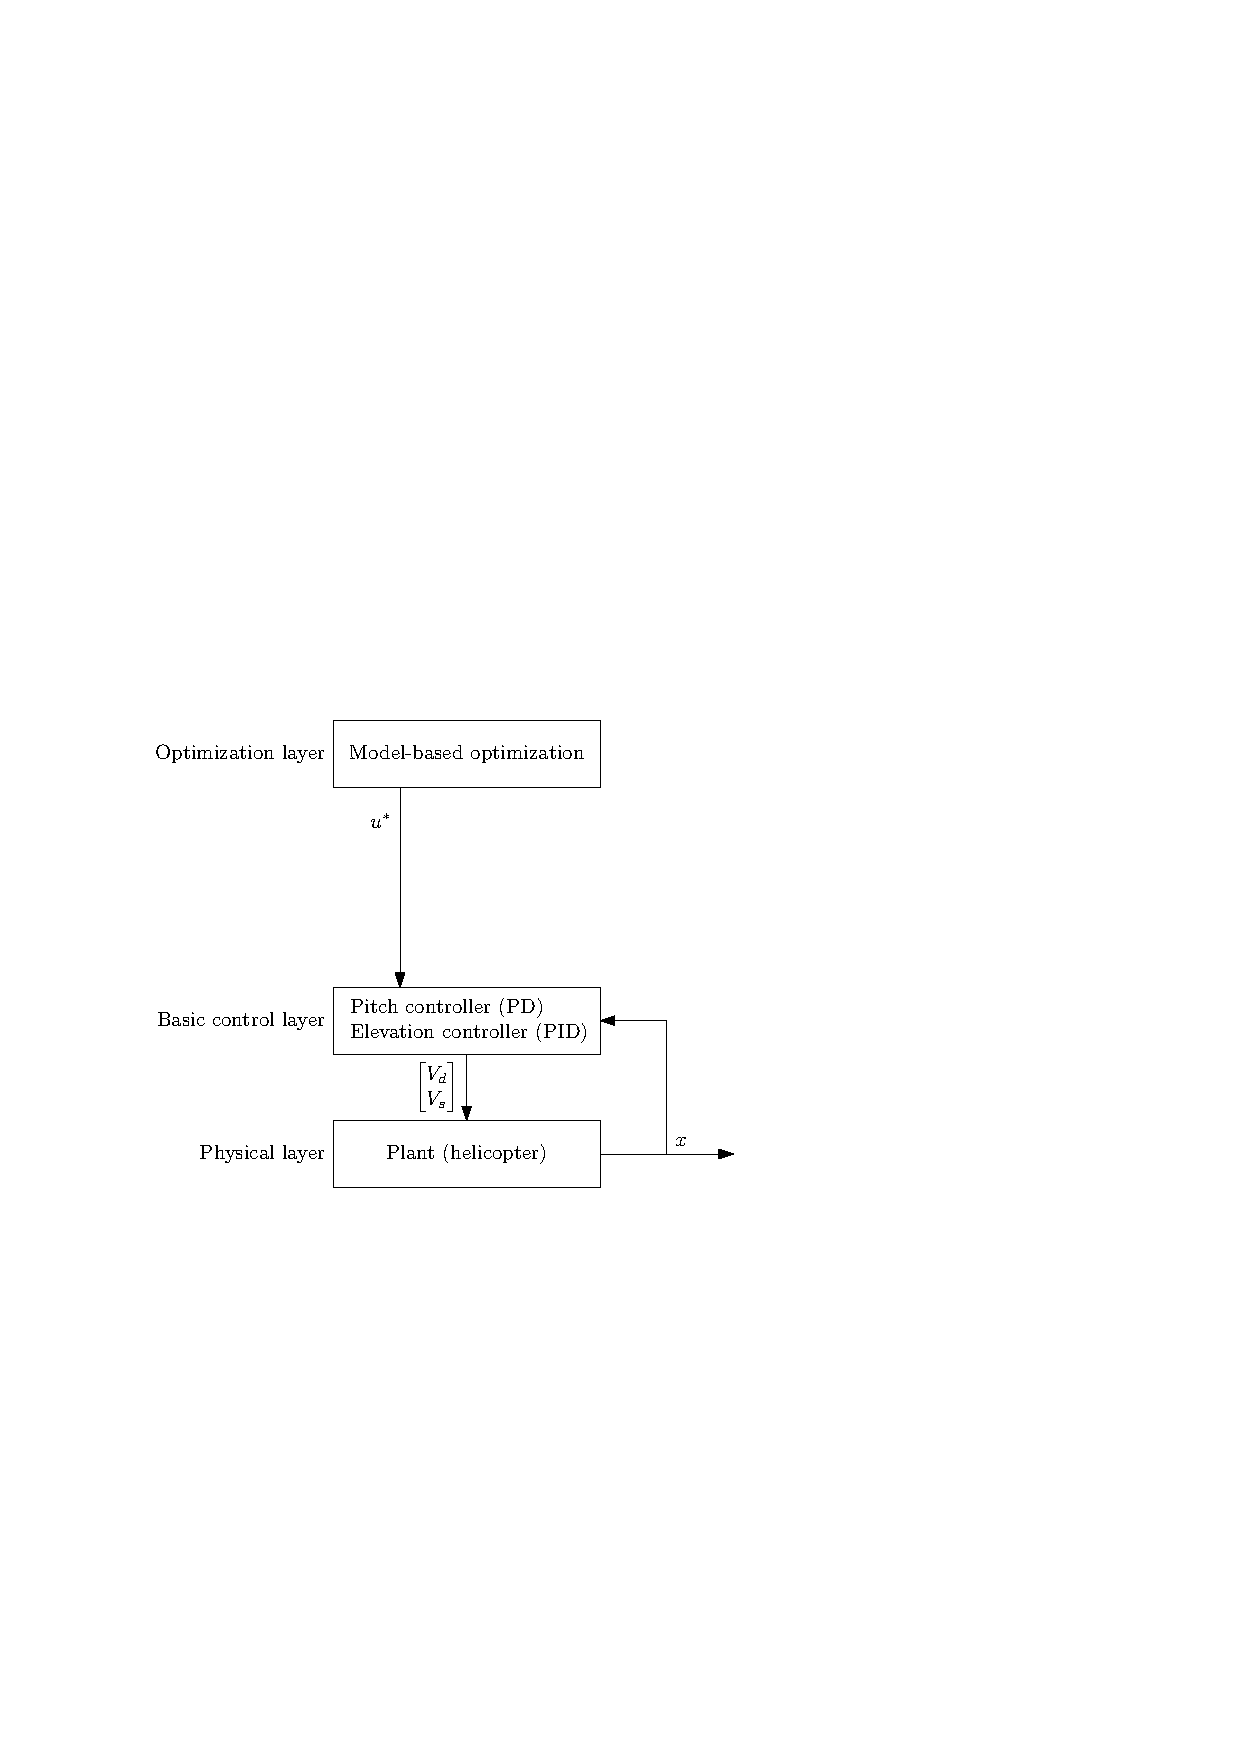
\includegraphics[width=1.00\textwidth]{figures/layers_openloop.pdf}
    \caption{Basic control hierarchy under open loop.}
\label{fig:layers_openloop}
\end{figure}
We start by writing the model on continuous time state space form.
\begin{equation}\label{eq:contineus_time_model}
    \vec{\dot{x}} = A_c\vec{x} + B_c u 
\end{equation}
Where $\vec{x}=\begin{bmatrix} \lambda&r&p&\dot{p} \end{bmatrix}^\top$ and $u=p_c$, further are $A_c$ and $B_c$ constructed from \cref{eq:model}. 
\begin{equation*}
A_c =
    \begin{bmatrix}
        0 &  1 &  0 & 0 \\
        0 &  0 &  -K_2 & 0  \\
        0 &  0 &  0 & 1 \\
        0 &  0 & -K_1K_{pp} & -K_1K_{pd}                                 
    \end{bmatrix}
    , \quad B_c = 
    \begin{bmatrix} 0 \\ 0 \\ 0 \\ K_1K_{pp} \end{bmatrix}
\end{equation*}
The model in \cref{eq:contineus_time_model} models the lower layers of the system including the process, sensors, actuators and the regulatory control. In \cref{fig:layers_openloop} this refers to the basic control layer, including the feedback loop and the physical layer. An important part of this layer structure is that the sampling frequency in the lower layers are higher than in the upper layers. As long as the lower layers have sufficiently higher frequency than the upper layers we can hide these lower layers and simply look at the helicopter and its basic controllers as a black box with input $u^*$ and output $\vec{x}$.\\
\\
We discretize the model using the forward Euler method:
\begin{align*}
    \vec{x_{k+1}} &= \vec{x_k} + h\vec{\dot{x}_k} \\
                  &= \vec{x_k} + h(A_c\vec{x_k} + B_c u_k) \\
                  &= \underbrace{(I + hA_C)}_{A}\vec{x_k} + \underbrace{hB_c}_{B} u_k \\
\end{align*}
Next we will calculate the optimal trajectory for moving the helicopter from $x_0 = \begin{bmatrix}\lambda_0 &0&0&0 \end{bmatrix}^\top$ to $x_f = \begin{bmatrix}\lambda_f &0&0&0 \end{bmatrix}^\top$ when the elevation angle is assumed to be constant. We will also implement the constraint 
\begin{equation}
    |p_k| \leq \frac{30\pi}{180},\quad k \in {1,\dots,N}
\end{equation}
Since the manipulated variable $p_c$ in this case is the setpoint for the $p$ controller, the constraint will also be implemented for the manipulated variable. We want to minimize the cost function 
\begin{equation}\label{eq:cost_function}
    \phi(\vec{z}) = \sum_{i=0}^{N-1}(\lambda_{i+1}-\lambda_f)^2 + rp_{ci}^2, \quad q\geq0
\end{equation}
Where $\vec{z}=\begin{bmatrix} \vec{x}_1^\top, \dots, \vec{x}_N^\top, {p_c}_{0}, \dots, {p_c}_{N-1} \end{bmatrix}^\top$. We use horizon $N = 100$, timestep $h=0.25$s, $\lambda_0 = \pi$ and $\lambda_f = 0$. 
Then cost function becomes:
\begin{equation}
    \phi(\vec{z}) = \sum_{i=0}^{N-1}\frac12\vec{x}_{i+1}^\top Q_{i+1} \vec{x}_{i+1}+ \frac12Rp_{ci}^2
\end{equation}
Where $$R = 2r, \quad Q_{i+1} = \begin{bmatrix} 2&0&0&0 \\0&0&0&0 \\0&0&0&0 \\0&0&0&0\end{bmatrix}$$
Finally we can rewrite the cost function to
\begin{equation}
    \phi(\vec{z}) = \frac12\vec{z}^\top G \vec{z}
\end{equation}
Where $G$ is a block diagonal matrix:
\begin{equation}
G = 
    \begin{bmatrix}
    Q_1 &0&\dots&\dots&\dots&0 \\
    0 &\ddots&\ddots&&&\vdots \\ 
    \vdots &\ddots&Q_N&\ddots&&\vdots \\ 
    \vdots &&\ddots&R_0&\ddots&\vdots \\ 
    \vdots &&&\ddots&\ddots&0 \\
    0&\dots&\dots&\dots&0&R_{N-1}
    \end{bmatrix}
\end{equation}
Next we write the model as an equality constraint:
\begin{equation}\label{eq:equality_constrains}
A_{eq}\vec{z}=b_{eq}
\end{equation}
Where $$A_{eq}= 
\left[
\begin{array}{ccccc|ccccc}
I & 0 & \dots & \dots & 0  &-B_0 &0&\dots&\dots&0\\
-A_1 & I &\ddots& & \vdots  &0 &\ddots&\ddots&&\vdots\\
0 &\ddots&\ddots&\ddots&\vdots  &\vdots &\ddots&\ddots&\ddots&\vdots\\
\vdots &\ddots&\ddots&\ddots&0&\vdots&&\ddots&\ddots&\vdots\\
0 &\dots&0&-A_N&I  & 0 &\dots&\dots&0&-B_N
\end{array}
\right]$$
and
\begin{equation*}
b_{eq} = \begin{bmatrix} A_0 \vec{x}_0 \\ 0 \\ \vdots \\ 0\end{bmatrix}
\end{equation*}
Then we solve the optimization problem using the MATLAB function quadprog. The resulting trajectory and manipulated variable are shown in \cref{fig:figure3,fig:figure1,fig:figure2}.
\begin{figure}[H] 
        \centering
        \setlength{\figureheight}{6cm}
        \setlength{\figurewidth}{10cm}
        % This file was created by matlab2tikz.
%
%The latest updates can be retrieved from
%  http://www.mathworks.com/matlabcentral/fileexchange/22022-matlab2tikz-matlab2tikz
%where you can also make suggestions and rate matlab2tikz.
%
\definecolor{mycolor1}{rgb}{1.00000,0.00000,1.00000}%
%
\begin{tikzpicture}

\begin{axis}[%
width=0.951\figurewidth,
height=\figureheight,
at={(0\figurewidth,0\figureheight)},
scale only axis,
every outer x axis line/.append style={black},
every x tick label/.append style={font=\color{black}},
xmin=4,
xmax=24,
xlabel={Time [s]},
every outer y axis line/.append style={black},
every y tick label/.append style={font=\color{black}},
ymin=-0.5,
ymax=3.5,
ylabel={$\text{u, }\lambda\text{ [rad]}$},
axis background/.style={fill=white},
xmajorgrids,
ymajorgrids,
legend style={legend cell align=left,align=left,draw=black}
]
\addplot[const plot,color=blue,solid] plot table[row sep=crcr] {%
0	0\\
0.25	0\\
0.5	0\\
0.75	0\\
1	0\\
1.25	0\\
1.5	0\\
1.75	0\\
2	0\\
2.25	0\\
2.5	0\\
2.75	0\\
3	0\\
3.25	0\\
3.5	0\\
3.75	0\\
4	0\\
4.25	0\\
4.5	0\\
4.75	0\\
5	0.523598775598287\\
5.25	0.523598775598265\\
5.5	0.523598775598189\\
5.75	0.523598775597489\\
6	0.523598775192491\\
6.25	0.481894292704602\\
6.5	0.383650233993971\\
6.75	0.294913191540567\\
7	0.215288098350692\\
7.25	0.14434491396085\\
7.5	0.0816258059381605\\
7.75	0.0266523817818906\\
8	-0.0210673560744442\\
8.25	-0.0620325480831923\\
8.5	-0.0967436272545484\\
8.75	-0.125697134040161\\
9	-0.149381207080167\\
9.25	-0.168271733662333\\
9.5	-0.182829127566075\\
9.75	-0.193495692730564\\
10	-0.200693526425264\\
10.25	-0.204822913698697\\
10.5	-0.206261164797922\\
10.75	-0.205361848322486\\
11	-0.202454374677314\\
11.25	-0.197843886644905\\
11.5	-0.191811416428943\\
11.75	-0.184614271208773\\
12	-0.17648661200487\\
12.25	-0.167640193430913\\
12.5	-0.158265234656145\\
12.75	-0.148531394590709\\
13	-0.138588826912946\\
13.25	-0.128569293063133\\
13.5	-0.118587313719309\\
13.75	-0.108741341537838\\
14	-0.0991149400770749\\
14.25	-0.0897779558226594\\
14.5	-0.0807876720950699\\
14.75	-0.0721899353437172\\
15	-0.0640202459180335\\
15.25	-0.0563048068570413\\
15.5	-0.0490615255582213\\
15.75	-0.042300964378454\\
16	-0.0360272372894621\\
16.25	-0.0302388506631704\\
16.5	-0.0249294871048105\\
16.75	-0.0200887319898338\\
17	-0.0157027430013568\\
17.25	-0.0117548635146715\\
17.5	-0.00822618114104298\\
17.75	-0.00509603313128463\\
18	-0.00234246065702036\\
18.25	5.73857594592064e-05\\
18.5	0.00212688720106961\\
18.75	0.00388964108933986\\
19	0.00536918699120902\\
19.25	0.00658877074028386\\
19.5	0.00757114409492629\\
19.75	0.00833839716814731\\
20	0.00891182090376196\\
20.25	0.00931179693548937\\
20.5	0.00955771224687396\\
20.75	0.00966789614658487\\
21	0.00965957718266085\\
21.25	0.00954885773774819\\
21.5	0.00935070417276009\\
21.75	0.00907895051637408\\
22	0.00874631383034659\\
22.25	0.00836441951397492\\
22.5	0.00794383494361481\\
22.75	0.00749410997361627\\
23	0.00702382295220371\\
23.25	0.00654063102869111\\
23.5	0.00605132364610325\\
23.75	0.00556187822496138\\
24	0.00507751714887783\\
24.25	0.00460276525978042\\
24.5	0.00414150715886401\\
24.75	0.00369704368700605\\
25	0.00327214702265253\\
25.25	0.00286911388165451\\
25.5	0.00248981632497306\\
25.75	0.00213574966479792\\
26	0.00180807688851424\\
26.25	0.00150766886324062\\
26.5	0.0012351392953996\\
26.75	0.000990872931732319\\
27	0.000775044704272603\\
27.25	0.000587626318550092\\
27.5	0.000428375030433439\\
27.75	0.000296796983864882\\
28	0.00019207467389022\\
28.25	0.000112945755860646\\
28.5	5.75212021345266e-05\\
28.75	2.30414127689544e-05\\
29	5.60489223336172e-06\\
29.25	-1.11674257890394e-18\\
29.5	-4.16914188487623e-19\\
29.75	0\\
30	0\\
30.25	0\\
30.5	0\\
30.75	0\\
31	0\\
31.25	0\\
31.5	0\\
31.75	0\\
32	0\\
32.25	0\\
32.5	0\\
32.75	0\\
33	0\\
33.25	0\\
33.5	0\\
33.75	0\\
34	0\\
34.25	0\\
34.5	0\\
34.75	0\\
35	0\\
};
\addlegendentry{$\text{p}_\text{c}$};

\addplot [color=mycolor1,solid]
  table[row sep=crcr]{%
0	3.14159265358979\\
0.25	3.14159265358979\\
0.5	3.14159265358979\\
0.75	3.14159265358979\\
1	3.14159265358979\\
1.25	3.14159265358979\\
1.5	3.14159265358979\\
1.75	3.14159265358979\\
2	3.14159265358979\\
2.25	3.14159265358979\\
2.5	3.14159265358979\\
2.75	3.14159265358979\\
3	3.14159265358979\\
3.25	3.14159265358979\\
3.5	3.14159265358979\\
3.75	3.14159265358979\\
4	3.14159265358979\\
4.25	3.14159265358979\\
4.5	3.14159265358979\\
4.75	3.14159265358979\\
5	3.14159265358979\\
5.25	3.14159265358979\\
5.5	3.14159265358979\\
5.75	3.14159265358979\\
6	3.13784214136253\\
6.25	3.126215553458\\
6.5	3.10330930002997\\
6.75	3.06662741519119\\
7	3.01445392239709\\
7.25	2.94595500428244\\
7.5	2.86143626200142\\
7.75	2.76212170563882\\
8	2.64983565255748\\
8.25	2.52672275133966\\
8.5	2.39503951330361\\
8.75	2.25701311663149\\
9	2.1147526767806\\
9.25	1.9701979310055\\
9.5	1.82509321660995\\
9.75	1.6809779266509\\
10	1.53918737930468\\
10.25	1.4008600700765\\
10.5	1.26694868416894\\
10.75	1.13823318449514\\
11	1.01533490071383\\
11.25	0.898730935265922\\
11.5	0.788768450736424\\
11.75	0.685678560720859\\
12	0.589589647401895\\
12.25	0.500539994619248\\
12.5	0.418489668699463\\
12.75	0.34333160894368\\
13	0.274901910497019\\
13.25	0.21298929742021\\
13.5	0.157343795030944\\
13.75	0.107684619133592\\
14	0.0637073063320437\\
14.25	0.0250901146825404\\
14.5	-0.00850027220186857\\
14.75	-0.0374037016223799\\
15	-0.0619621308425424\\
15.25	-0.0825157894017468\\
15.5	-0.099399884680409\\
15.75	-0.112941810525984\\
16	-0.123458819020861\\
16.25	-0.131256116126597\\
16.5	-0.136625342912986\\
16.75	-0.139843405320009\\
17	-0.141171616856007\\
17.25	-0.140855120261473\\
17.5	-0.139122555924201\\
17.75	-0.136185946682111\\
18	-0.132240770562594\\
18.25	-0.127466194953525\\
18.5	-0.122025447656233\\
18.75	-0.116066302213293\\
19	-0.109721656815576\\
19.25	-0.103110187958028\\
19.5	-0.0963370618191989\\
19.75	-0.0894946880750038\\
20	-0.082663502514325\\
20.25	-0.0759127663962628\\
20.5	-0.06930137197162\\
20.75	-0.0628786449813556\\
21	-0.0566851362406178\\
21.25	-0.0507533956180339\\
21.5	-0.0451087228267689\\
21.75	-0.0397698904578883\\
22	-0.0347498356100031\\
22.25	-0.0300563173048605\\
22.5	-0.0256925376298312\\
22.75	-0.0216577252188954\\
23	-0.0179476802778117\\
23.25	-0.0145552808809667\\
23.5	-0.0114709507213921\\
23.75	-0.00868308888612273\\
24	-0.00617846256099546\\
24.25	-0.00394256384666598\\
24.5	-0.00195993209547086\\
24.75	-0.000214443361099672\\
25	0.00131043130599011\\
25.25	0.00263139688092275\\
25.5	0.0037651327981449\\
25.75	0.00472811685051908\\
26	0.00553647259514227\\
26.25	0.00620583831900822\\
26.5	0.00675125565149537\\
26.75	0.00718707596514325\\
27	0.00752688278080753\\
27.25	0.0077834284891175\\
27.5	0.00796858382057109\\
27.75	0.00809329864847639\\
28	0.00816757290445425\\
28.25	0.00820043664527305\\
28.5	0.00819993866319176\\
28.75	0.00817314352458638\\
29	0.00812613761355793\\
29.25	0.00806404571782923\\
29.5	0.00799106097605194\\
29.75	0.0079104925694888\\
30	0.00782483707002407\\
30.25	0\\
30.5	0\\
30.75	0\\
31	0\\
31.25	0\\
31.5	0\\
31.75	0\\
32	0\\
32.25	0\\
32.5	0\\
32.75	0\\
33	0\\
33.25	0\\
33.5	0\\
33.75	0\\
34	0\\
34.25	0\\
34.5	0\\
34.75	0\\
35	0\\
};
\addlegendentry{$\lambda$};

\addplot [color=mycolor1,solid,forget plot]
  table[row sep=crcr]{%
0	3.14159265358979\\
0.25	3.14159265358979\\
0.5	3.14159265358979\\
0.75	3.14159265358979\\
1	3.14159265358979\\
1.25	3.14159265358979\\
1.5	3.14159265358979\\
1.75	3.14159265358979\\
2	3.14159265358979\\
2.25	3.14159265358979\\
2.5	3.14159265358979\\
2.75	3.14159265358979\\
3	3.14159265358979\\
3.25	3.14159265358979\\
3.5	3.14159265358979\\
3.75	3.14159265358979\\
4	3.14159265358979\\
4.25	3.14159265358979\\
4.5	3.14159265358979\\
4.75	3.14159265358979\\
5	3.14159265358979\\
5.25	3.14159265358979\\
5.5	3.14159265358979\\
5.75	3.14159265358979\\
6	3.13784214136253\\
6.25	3.126215553458\\
6.5	3.10330930002997\\
6.75	3.06662741519119\\
7	3.01445392239709\\
7.25	2.94595500428244\\
7.5	2.86143626200142\\
7.75	2.76212170563882\\
8	2.64983565255748\\
8.25	2.52672275133966\\
8.5	2.39503951330361\\
8.75	2.25701311663149\\
9	2.1147526767806\\
9.25	1.9701979310055\\
9.5	1.82509321660995\\
9.75	1.6809779266509\\
10	1.53918737930468\\
10.25	1.4008600700765\\
10.5	1.26694868416894\\
10.75	1.13823318449514\\
11	1.01533490071383\\
11.25	0.898730935265922\\
11.5	0.788768450736424\\
11.75	0.685678560720859\\
12	0.589589647401895\\
12.25	0.500539994619248\\
12.5	0.418489668699463\\
12.75	0.34333160894368\\
13	0.274901910497019\\
13.25	0.21298929742021\\
13.5	0.157343795030944\\
13.75	0.107684619133592\\
14	0.0637073063320437\\
14.25	0.0250901146825404\\
14.5	-0.00850027220186857\\
14.75	-0.0374037016223799\\
15	-0.0619621308425424\\
15.25	-0.0825157894017468\\
15.5	-0.099399884680409\\
15.75	-0.112941810525984\\
16	-0.123458819020861\\
16.25	-0.131256116126597\\
16.5	-0.136625342912986\\
16.75	-0.139843405320009\\
17	-0.141171616856007\\
17.25	-0.140855120261473\\
17.5	-0.139122555924201\\
17.75	-0.136185946682111\\
18	-0.132240770562594\\
18.25	-0.127466194953525\\
18.5	-0.122025447656233\\
18.75	-0.116066302213293\\
19	-0.109721656815576\\
19.25	-0.103110187958028\\
19.5	-0.0963370618191989\\
19.75	-0.0894946880750038\\
20	-0.082663502514325\\
20.25	-0.0759127663962628\\
20.5	-0.06930137197162\\
20.75	-0.0628786449813556\\
21	-0.0566851362406178\\
21.25	-0.0507533956180339\\
21.5	-0.0451087228267689\\
21.75	-0.0397698904578883\\
22	-0.0347498356100031\\
22.25	-0.0300563173048605\\
22.5	-0.0256925376298312\\
22.75	-0.0216577252188954\\
23	-0.0179476802778117\\
23.25	-0.0145552808809667\\
23.5	-0.0114709507213921\\
23.75	-0.00868308888612273\\
24	-0.00617846256099546\\
24.25	-0.00394256384666598\\
24.5	-0.00195993209547086\\
24.75	-0.000214443361099672\\
25	0.00131043130599011\\
25.25	0.00263139688092275\\
25.5	0.0037651327981449\\
25.75	0.00472811685051908\\
26	0.00553647259514227\\
26.25	0.00620583831900822\\
26.5	0.00675125565149537\\
26.75	0.00718707596514325\\
27	0.00752688278080753\\
27.25	0.0077834284891175\\
27.5	0.00796858382057109\\
27.75	0.00809329864847639\\
28	0.00816757290445425\\
28.25	0.00820043664527305\\
28.5	0.00819993866319176\\
28.75	0.00817314352458638\\
29	0.00812613761355793\\
29.25	0.00806404571782923\\
29.5	0.00799106097605194\\
29.75	0.0079104925694888\\
30	0.00782483707002407\\
30.25	0\\
30.5	0\\
30.75	0\\
31	0\\
31.25	0\\
31.5	0\\
31.75	0\\
32	0\\
32.25	0\\
32.5	0\\
32.75	0\\
33	0\\
33.25	0\\
33.5	0\\
33.75	0\\
34	0\\
34.25	0\\
34.5	0\\
34.75	0\\
35	0\\
};
\end{axis}
\end{tikzpicture}%
        \caption{Optimal trajectory and input using weight $r=1$} 
\label{fig:figure3} 
\end{figure}
\begin{figure}[H] 
        \centering
        \setlength{\figureheight}{6cm}
        \setlength{\figurewidth}{10cm}
        % This file was created by matlab2tikz.
%
%The latest updates can be retrieved from
%  http://www.mathworks.com/matlabcentral/fileexchange/22022-matlab2tikz-matlab2tikz
%where you can also make suggestions and rate matlab2tikz.
%
\definecolor{mycolor1}{rgb}{1.00000,0.00000,1.00000}%
%
\begin{tikzpicture}

\begin{axis}[%
width=0.951\figurewidth,
height=\figureheight,
at={(0\figurewidth,0\figureheight)},
scale only axis,
every outer x axis line/.append style={black},
every x tick label/.append style={font=\color{black}},
xmin=0,
xmax=35,
xlabel={Time [s]},
every outer y axis line/.append style={black},
every y tick label/.append style={font=\color{black}},
ymin=-1,
ymax=3.5,
ylabel={$\text{u, }\lambda\text{ [rad]}$},
axis background/.style={fill=white},
title={Weight q = 0.1},
axis x line*=bottom,
axis y line*=left,
legend style={legend cell align=left,align=left,draw=black}
]
\addplot[const plot,color=blue,solid] plot table[row sep=crcr] {%
0	0\\
0.25	0\\
0.5	0\\
0.75	0\\
1	0\\
1.25	0\\
1.5	0\\
1.75	0\\
2	0\\
2.25	0\\
2.5	0\\
2.75	0\\
3	0\\
3.25	0\\
3.5	0\\
3.75	0\\
4	0\\
4.25	0\\
4.5	0\\
4.75	0\\
5	0.523598775598074\\
5.25	0.523598775598034\\
5.5	0.523598775597983\\
5.75	0.523598775597915\\
6	0.523598775597823\\
6.25	0.523598775597692\\
6.5	0.523598775597497\\
6.75	0.523598775597182\\
7	0.523598775596606\\
7.25	0.523598775595267\\
7.5	0.523598775589254\\
7.75	0.388605461895739\\
8	0.10951698887527\\
8.25	-0.110038339461022\\
8.5	-0.276911237552916\\
8.75	-0.397906827316469\\
9	-0.479636751279011\\
9.25	-0.523591909441963\\
9.5	-0.523598775343426\\
9.75	-0.523598775363433\\
10	-0.523598722414531\\
10.25	-0.503434893916266\\
10.5	-0.464970440433064\\
10.75	-0.420773458613526\\
11	-0.373478625554464\\
11.25	-0.32522986550994\\
11.5	-0.277723446822207\\
11.75	-0.23225530276674\\
12	-0.189770188173245\\
12.25	-0.150910740882838\\
12.5	-0.116064946577637\\
12.75	-0.0854108906849835\\
13	-0.0589580160110363\\
13.25	-0.0365843889433275\\
13.5	-0.0180697126514252\\
13.75	-0.00312401628611978\\
14	0.0085879009858575\\
14.25	0.0174260785786064\\
14.5	0.0237587809673789\\
14.75	0.0279493320089856\\
15	0.0303460343335946\\
15.25	0.0312747968277704\\
15.5	0.0310340938210644\\
15.75	0.0298918916543043\\
16	0.0280841989107185\\
16.25	0.0258149231897645\\
16.5	0.0232567477403919\\
16.75	0.0205527737516956\\
17	0.0178187071682619\\
17.25	0.0151454014055185\\
17.5	0.0126015984112879\\
17.75	0.0102367395172331\\
18	0.00808374401737152\\
18.25	0.00616167714278127\\
18.5	0.00447824995691099\\
18.75	0.00303211167359721\\
19	0.00181491008787609\\
19.25	0.000813108362100164\\
19.5	9.55652768421745e-06\\
19.75	-0.000615176022881656\\
20	-0.00108169482085181\\
20.25	-0.00141088489524046\\
20.5	-0.00162320634848339\\
20.75	-0.00173816006303826\\
21	-0.00177390207933103\\
21.25	-0.00174698538733233\\
21.5	-0.00167220868418209\\
21.75	-0.00156255290812047\\
22	-0.0014291879259838\\
22.25	-0.00128153351051757\\
22.5	-0.00112736059780635\\
22.75	-0.000972920686000228\\
23	-0.000823093062976664\\
23.25	-0.000681541286448394\\
23.5	-0.000550871952314935\\
23.75	-0.000432790254030426\\
24	-0.000328248145159256\\
24.25	-0.000237582064620324\\
24.5	-0.000160638171127123\\
24.75	-9.68838666457343e-05\\
25	-4.55050786779726e-05\\
25.25	-5.48933099237643e-06\\
25.5	2.43049226562372e-05\\
25.75	4.50918802708431e-05\\
26	5.8113799538616e-05\\
26.25	6.46069335734721e-05\\
26.5	6.57765222737536e-05\\
26.75	6.27792011280751e-05\\
27	5.67109984837793e-05\\
27.25	4.85988379814542e-05\\
27.5	3.93931031714662e-05\\
27.75	2.99583230120062e-05\\
28	2.10584099342284e-05\\
28.25	1.33322661490434e-05\\
28.5	7.25543918037023e-06\\
28.75	3.08509956999618e-06\\
29	7.91904987941527e-07\\
29.25	-4.05937439716459e-17\\
29.5	-1.53321449279011e-17\\
29.75	0\\
30	0\\
30.25	0\\
30.5	0\\
30.75	0\\
31	0\\
31.25	0\\
31.5	0\\
31.75	0\\
32	0\\
32.25	0\\
32.5	0\\
32.75	0\\
33	0\\
33.25	0\\
33.5	0\\
33.75	0\\
34	0\\
34.25	0\\
34.5	0\\
34.75	0\\
35	0\\
};
\addlegendentry{$\text{p}_\text{c}$};

\addplot [color=mycolor1,solid]
  table[row sep=crcr]{%
0	3.14159265358979\\
0.25	3.14159265358979\\
0.5	3.14159265358979\\
0.75	3.14159265358979\\
1	3.14159265358979\\
1.25	3.14159265358979\\
1.5	3.14159265358979\\
1.75	3.14159265358979\\
2	3.14159265358979\\
2.25	3.14159265358979\\
2.5	3.14159265358979\\
2.75	3.14159265358979\\
3	3.14159265358979\\
3.25	3.14159265358979\\
3.5	3.14159265358979\\
3.75	3.14159265358979\\
4	3.14159265358979\\
4.25	3.14159265358979\\
4.5	3.14159265358979\\
4.75	3.14159265358979\\
5	3.14159265358979\\
5.25	3.14159265358979\\
5.5	3.14159265358979\\
5.75	3.14159265358979\\
6	3.13784214136253\\
6.25	3.126215553458\\
6.5	3.10330930002998\\
6.75	3.06662741519122\\
7	3.01445392239423\\
7.25	2.94565627711768\\
7.5	2.85950776329371\\
7.75	2.75555158796541\\
8	2.63350511049065\\
8.25	2.49319560603263\\
8.5	2.33451857606511\\
8.75	2.15837827192605\\
9	1.96780007787047\\
9.25	1.76741104454662\\
9.5	1.56258105127613\\
9.75	1.35868396793868\\
10	1.16059209032489\\
10.25	0.972354196797713\\
10.5	0.796950123259841\\
10.75	0.636432933749591\\
11	0.492159597969274\\
11.25	0.36485729820996\\
11.5	0.25463993267206\\
11.75	0.161096235930179\\
12	0.0834005912521931\\
12.25	0.0204236245333906\\
12.5	-0.0291675128159417\\
12.75	-0.0668230046530649\\
13	-0.0940391853047939\\
13.25	-0.112301690219796\\
13.5	-0.123041675965191\\
13.75	-0.127603583533352\\
14	-0.127222853792057\\
14.25	-0.123012039483811\\
14.5	-0.115953847476759\\
14.75	-0.106899763407816\\
15	-0.0965730445362397\\
15.25	-0.0855750068726116\\
15.5	-0.0743936735427865\\
15.75	-0.0634139886026101\\
16	-0.0529289309785858\\
16.25	-0.0431509845929514\\
16.5	-0.034223531491126\\
16.75	-0.0262318339987593\\
17	-0.0192133591912855\\
17.25	-0.0131672742880113\\
17.5	-0.00806300535517535\\
17.75	-0.00384780454936746\\
18	-0.0004533138735938\\
18.25	0.00219885300364836\\
18.5	0.0041924638884134\\
18.75	0.00561289086980216\\
19	0.00654412528516249\\
19.25	0.00706650021892946\\
19.5	0.00725503299040899\\
19.75	0.00717830051005529\\
20	0.00689776339525422\\
20.25	0.00646745966611192\\
20.5	0.00593399511017771\\
20.75	0.00533676452114737\\
21	0.00470834557251294\\
21.25	0.00407501475230339\\
21.5	0.00345734229922592\\
21.75	0.00287083024602222\\
22	0.00232656434980062\\
22.25	0.00183185677553755\\
22.5	0.00139086184134206\\
22.75	0.00100515190830851\\
23	0.000674244605617742\\
23.25	0.0003960760448359\\
23.5	0.000167417532882236\\
23.75	-1.57644118584706e-05\\
24	-0.000158003147386422\\
24.25	-0.000264079167713\\
24.5	-0.000338815653456829\\
24.75	-0.000386917817245833\\
25	-0.000412851210807727\\
25.25	-0.000420754050890027\\
25.5	-0.000414378691834756\\
25.75	-0.000397057581793275\\
26	-0.000371689350269946\\
26.25	-0.000340741054982522\\
26.5	-0.000306263038766121\\
26.75	-0.000269913289732788\\
27	-0.00023298864146416\\
27.25	-0.00019646057949526\\
27.5	-0.000161013823462394\\
27.75	-0.000127086220927492\\
28	-9.49088102821858e-05\\
28.25	-6.45451778638679e-05\\
28.5	-3.5929439305405e-05\\
28.75	-8.90230607054183e-06\\
29	1.67552588483429e-05\\
29.25	4.12913533646134e-05\\
29.5	6.49561545002824e-05\\
29.75	8.79796792978908e-05\\
30	0.00011055569399486\\
30.25	0\\
30.5	0\\
30.75	0\\
31	0\\
31.25	0\\
31.5	0\\
31.75	0\\
32	0\\
32.25	0\\
32.5	0\\
32.75	0\\
33	0\\
33.25	0\\
33.5	0\\
33.75	0\\
34	0\\
34.25	0\\
34.5	0\\
34.75	0\\
35	0\\
};
\addlegendentry{$\lambda$};

\addplot [color=mycolor1,solid,forget plot]
  table[row sep=crcr]{%
0	3.14159265358979\\
0.25	3.14159265358979\\
0.5	3.14159265358979\\
0.75	3.14159265358979\\
1	3.14159265358979\\
1.25	3.14159265358979\\
1.5	3.14159265358979\\
1.75	3.14159265358979\\
2	3.14159265358979\\
2.25	3.14159265358979\\
2.5	3.14159265358979\\
2.75	3.14159265358979\\
3	3.14159265358979\\
3.25	3.14159265358979\\
3.5	3.14159265358979\\
3.75	3.14159265358979\\
4	3.14159265358979\\
4.25	3.14159265358979\\
4.5	3.14159265358979\\
4.75	3.14159265358979\\
5	3.14159265358979\\
5.25	3.14159265358979\\
5.5	3.14159265358979\\
5.75	3.14159265358979\\
6	3.13784214136253\\
6.25	3.126215553458\\
6.5	3.10330930002998\\
6.75	3.06662741519122\\
7	3.01445392239423\\
7.25	2.94565627711768\\
7.5	2.85950776329371\\
7.75	2.75555158796541\\
8	2.63350511049065\\
8.25	2.49319560603263\\
8.5	2.33451857606511\\
8.75	2.15837827192605\\
9	1.96780007787047\\
9.25	1.76741104454662\\
9.5	1.56258105127613\\
9.75	1.35868396793868\\
10	1.16059209032489\\
10.25	0.972354196797713\\
10.5	0.796950123259841\\
10.75	0.636432933749591\\
11	0.492159597969274\\
11.25	0.36485729820996\\
11.5	0.25463993267206\\
11.75	0.161096235930179\\
12	0.0834005912521931\\
12.25	0.0204236245333906\\
12.5	-0.0291675128159417\\
12.75	-0.0668230046530649\\
13	-0.0940391853047939\\
13.25	-0.112301690219796\\
13.5	-0.123041675965191\\
13.75	-0.127603583533352\\
14	-0.127222853792057\\
14.25	-0.123012039483811\\
14.5	-0.115953847476759\\
14.75	-0.106899763407816\\
15	-0.0965730445362397\\
15.25	-0.0855750068726116\\
15.5	-0.0743936735427865\\
15.75	-0.0634139886026101\\
16	-0.0529289309785858\\
16.25	-0.0431509845929514\\
16.5	-0.034223531491126\\
16.75	-0.0262318339987593\\
17	-0.0192133591912855\\
17.25	-0.0131672742880113\\
17.5	-0.00806300535517535\\
17.75	-0.00384780454936746\\
18	-0.0004533138735938\\
18.25	0.00219885300364836\\
18.5	0.0041924638884134\\
18.75	0.00561289086980216\\
19	0.00654412528516249\\
19.25	0.00706650021892946\\
19.5	0.00725503299040899\\
19.75	0.00717830051005529\\
20	0.00689776339525422\\
20.25	0.00646745966611192\\
20.5	0.00593399511017771\\
20.75	0.00533676452114737\\
21	0.00470834557251294\\
21.25	0.00407501475230339\\
21.5	0.00345734229922592\\
21.75	0.00287083024602222\\
22	0.00232656434980062\\
22.25	0.00183185677553755\\
22.5	0.00139086184134206\\
22.75	0.00100515190830851\\
23	0.000674244605617742\\
23.25	0.0003960760448359\\
23.5	0.000167417532882236\\
23.75	-1.57644118584706e-05\\
24	-0.000158003147386422\\
24.25	-0.000264079167713\\
24.5	-0.000338815653456829\\
24.75	-0.000386917817245833\\
25	-0.000412851210807727\\
25.25	-0.000420754050890027\\
25.5	-0.000414378691834756\\
25.75	-0.000397057581793275\\
26	-0.000371689350269946\\
26.25	-0.000340741054982522\\
26.5	-0.000306263038766121\\
26.75	-0.000269913289732788\\
27	-0.00023298864146416\\
27.25	-0.00019646057949526\\
27.5	-0.000161013823462394\\
27.75	-0.000127086220927492\\
28	-9.49088102821858e-05\\
28.25	-6.45451778638679e-05\\
28.5	-3.5929439305405e-05\\
28.75	-8.90230607054183e-06\\
29	1.67552588483429e-05\\
29.25	4.12913533646134e-05\\
29.5	6.49561545002824e-05\\
29.75	8.79796792978908e-05\\
30	0.00011055569399486\\
30.25	0\\
30.5	0\\
30.75	0\\
31	0\\
31.25	0\\
31.5	0\\
31.75	0\\
32	0\\
32.25	0\\
32.5	0\\
32.75	0\\
33	0\\
33.25	0\\
33.5	0\\
33.75	0\\
34	0\\
34.25	0\\
34.5	0\\
34.75	0\\
35	0\\
};
\end{axis}
\end{tikzpicture}%
        \caption{Optimal trajectory and input using weight $r=1$} 
\label{fig:figure1}
\end{figure}
\begin{figure}[H] 
        \centering
        \setlength{\figureheight}{6cm}
        \setlength{\figurewidth}{10cm}
        % This file was created by matlab2tikz.
%
%The latest updates can be retrieved from
%  http://www.mathworks.com/matlabcentral/fileexchange/22022-matlab2tikz-matlab2tikz
%where you can also make suggestions and rate matlab2tikz.
%
\definecolor{mycolor1}{rgb}{1.00000,0.00000,1.00000}%
%
\begin{tikzpicture}

\begin{axis}[%
width=0.951\figurewidth,
height=\figureheight,
at={(0\figurewidth,0\figureheight)},
scale only axis,
every outer x axis line/.append style={black},
every x tick label/.append style={font=\color{black}},
xmin=0,
xmax=35,
xlabel={Time [s]},
every outer y axis line/.append style={black},
every y tick label/.append style={font=\color{black}},
ymin=-1,
ymax=3.5,
ylabel={$\text{u, }\lambda\text{ [rad]}$},
axis background/.style={fill=white},
title={Weight q = 0.1},
axis x line*=bottom,
axis y line*=left,
legend style={legend cell align=left,align=left,draw=black}
]
\addplot[const plot,color=blue,solid] plot table[row sep=crcr] {%
0	0\\
0.25	0\\
0.5	0\\
0.75	0\\
1	0\\
1.25	0\\
1.5	0\\
1.75	0\\
2	0\\
2.25	0\\
2.5	0\\
2.75	0\\
3	0\\
3.25	0\\
3.5	0\\
3.75	0\\
4	0\\
4.25	0\\
4.5	0\\
4.75	0\\
5	0.523598775615169\\
5.25	0.5235987755964\\
5.5	0.523598775594549\\
5.75	0.52359877559331\\
6	0.523598775594153\\
6.25	0.523598775595899\\
6.5	0.523598775593978\\
6.75	0.523598775592185\\
7	0.523598775591746\\
7.25	0.523598775587507\\
7.5	0.523598775602952\\
7.75	0.523598775558179\\
8	0.523598775566759\\
8.25	-0.0111206478957404\\
8.5	-0.523598775344135\\
8.75	-0.523598775500856\\
9	-0.523598775526942\\
9.25	-0.523598775537819\\
9.5	-0.523598775544247\\
9.75	-0.523598775550429\\
10	-0.523598775558698\\
10.25	-0.523598775561775\\
10.5	-0.523598775540568\\
10.75	-0.523598775532572\\
11	-0.5235987755984\\
11.25	-0.523598775524838\\
11.5	-0.523598775594557\\
11.75	-0.523594769592384\\
12	-0.320898640974965\\
12.25	-0.139657390682654\\
12.5	-0.00806732286835657\\
12.75	0.079999458244962\\
13	0.131930472749672\\
13.25	0.155493669232079\\
13.5	0.158156965996792\\
13.75	0.146618544042565\\
14	0.126532011621718\\
14.25	0.102394663770725\\
14.5	0.0775605031392445\\
14.75	0.0543396216989834\\
15	0.0341495037226155\\
15.25	0.0176898792191529\\
15.5	0.00511954617584905\\
15.75	-0.00377983999883833\\
16	-0.00946220265351182\\
16.25	-0.012502144311573\\
16.5	-0.013507533376759\\
16.75	-0.0130578689764999\\
17	-0.0116651393211352\\
17.25	-0.00975309280915269\\
17.5	-0.00765064071874683\\
17.75	-0.00559533009845749\\
18	-0.00374331114850426\\
18.25	-0.00218284833906498\\
18.5	-0.000949091509012456\\
18.75	-3.84630417437901e-05\\
19	0.000578414520583257\\
19.25	0.000945853410079653\\
19.5	0.00111453229328056\\
19.75	0.00113519077697364\\
20	0.00105437507048022\\
20.25	0.000911920963119002\\
20.5	0.000739817630183794\\
20.75	0.000562096794284886\\
21	0.000395422118694741\\
21.25	0.000250101295514519\\
21.5	0.000131298521694773\\
21.75	4.02808281264857e-05\\
22	-2.44167900699339e-05\\
22.25	-6.59781980555287e-05\\
22.5	-8.84799007346225e-05\\
22.75	-9.62597605719328e-05\\
23	-9.34697643697277e-05\\
23.25	-8.3790140056167e-05\\
23.5	-7.02760605148161e-05\\
23.75	-5.53064855364679e-05\\
24	-4.06060982376108e-05\\
24.25	-2.73146636145459e-05\\
24.5	-1.60825520061424e-05\\
24.75	-7.17592050694677e-06\\
25	-5.79625295616829e-07\\
25.25	3.9099790641874e-06\\
25.5	6.60678967412083e-06\\
25.75	7.87302304410315e-06\\
26	8.07342226545293e-06\\
26.25	7.54412794325329e-06\\
26.5	6.57398662004059e-06\\
26.75	5.3957525791655e-06\\
27	4.184641568288e-06\\
27.25	3.06191661249471e-06\\
27.5	2.10154101434737e-06\\
27.75	1.33835403330324e-06\\
28	7.76660145365087e-07\\
28.25	3.98537499279302e-07\\
28.5	1.71539160213463e-07\\
28.75	5.57565367773066e-08\\
29	1.03963969109549e-08\\
29.25	2.1862849533675e-13\\
29.5	2.17932395713985e-13\\
29.75	0\\
30	0\\
30.25	0\\
30.5	0\\
30.75	0\\
31	0\\
31.25	0\\
31.5	0\\
31.75	0\\
32	0\\
32.25	0\\
32.5	0\\
32.75	0\\
33	0\\
33.25	0\\
33.5	0\\
33.75	0\\
34	0\\
34.25	0\\
34.5	0\\
34.75	0\\
35	0\\
};
\addlegendentry{$\text{p}_\text{c}$};

\addplot [color=mycolor1,solid]
  table[row sep=crcr]{%
0	3.14159265358979\\
0.25	3.14159265358979\\
0.5	3.14159265358979\\
0.75	3.14159265358979\\
1	3.14159265358979\\
1.25	3.14159265358979\\
1.5	3.14159265358979\\
1.75	3.14159265358979\\
2	3.14159265358979\\
2.25	3.14159265358979\\
2.5	3.14159265358979\\
2.75	3.14159265358979\\
3	3.14159265358979\\
3.25	3.14159265358979\\
3.5	3.14159265358979\\
3.75	3.14159265358979\\
4	3.14159265358979\\
4.25	3.14159265358979\\
4.5	3.14159265358979\\
4.75	3.14159265358979\\
5	3.14159265358979\\
5.25	3.14159265358979\\
5.5	3.14159265358979\\
5.75	3.14159265358979\\
6	3.13784214135351\\
6.25	3.12621555344874\\
6.5	3.10330930002041\\
6.75	3.06662741518133\\
7	3.01445392238407\\
7.25	2.94565627710731\\
7.5	2.85950776328322\\
7.75	2.7555515879549\\
8	2.63350511048026\\
8.25	2.49319560602253\\
8.5	2.33451857605534\\
8.75	2.15741132146317\\
9	1.96183648402309\\
9.25	1.75160210505222\\
9.5	1.53457918643444\\
9.75	1.31827389774468\\
10	1.10856204744569\\
10.25	0.909636408550166\\
10.5	0.72433159931212\\
10.75	0.55449738597468\\
11	0.401311039383504\\
11.25	0.265508003180292\\
11.5	0.147541140939951\\
11.75	0.0476861308932072\\
12	-0.0338907721370796\\
12.25	-0.0970900805110839\\
12.5	-0.141852649908414\\
12.75	-0.168143545282482\\
13	-0.177394131619615\\
13.25	-0.172487700400851\\
13.5	-0.157105457518113\\
13.75	-0.135055351792788\\
14	-0.109784541443894\\
14.25	-0.084101778009114\\
14.5	-0.0600729998821311\\
14.75	-0.0390384428079875\\
15	-0.0217035409002521\\
15.25	-0.00826595573777884\\
15.5	0.00144816463085163\\
15.75	0.00785618000926249\\
16	0.0115092167862538\\
16.25	0.0130051621281167\\
16.5	0.0129250168612969\\
16.75	0.0117907668916998\\
17	0.0100415464494962\\
17.25	0.00802427740362974\\
17.5	0.00599493725764129\\
17.75	0.00412693647613014\\
18	0.00252361732144517\\
18.25	0.00123250372168697\\
18.5	0.000259551202688492\\
18.75	-0.000417787234074236\\
19	-0.000839380754015216\\
19.25	-0.00105344249024256\\
19.5	-0.00110978380601299\\
19.75	-0.00105513551498004\\
20	-0.000930252238357377\\
20.25	-0.000768459935008318\\
20.5	-0.00059529712529346\\
20.75	-0.00042892305475397\\
21	-0.000281008612152943\\
21.25	-0.000157878211602527\\
21.5	-6.17254970824858e-05\\
21.75	8.22266388802954e-06\\
22	5.46741768295492e-05\\
22.25	8.14147911343963e-05\\
22.5	9.26406681285736e-05\\
22.75	9.24743513332887e-05\\
23	8.46447256716714e-05\\
23.25	7.23041974613017e-05\\
23.5	5.79536045497031e-05\\
23.75	4.34459924107159e-05\\
24	3.00432230113797e-05\\
24.25	1.85034635876441e-05\\
24.5	9.182184168228e-06\\
24.75	2.13382986796054e-06\\
25	-2.79453752033704e-06\\
25.25	-5.88282556301574e-06\\
25.5	-7.47312383733555e-06\\
25.75	-7.92085660198151e-06\\
26	-7.56075738192696e-06\\
26.25	-6.68567603117707e-06\\
26.5	-5.53580761933637e-06\\
26.75	-4.29584960936392e-06\\
27	-3.09774565170643e-06\\
27.25	-2.02697147016321e-06\\
27.5	-1.1306883321627e-06\\
27.75	-4.26477593054087e-07\\
28	8.92626681643844e-08\\
28.25	4.33854948119525e-07\\
28.5	6.32143535081129e-07\\
28.75	7.11683761652601e-07\\
29	6.99294482135752e-07\\
29.25	6.18849422030505e-07\\
29.5	4.90122953876991e-07\\
29.75	3.28474430731669e-07\\
30	1.45142305709818e-07\\
30.25	0\\
30.5	0\\
30.75	0\\
31	0\\
31.25	0\\
31.5	0\\
31.75	0\\
32	0\\
32.25	0\\
32.5	0\\
32.75	0\\
33	0\\
33.25	0\\
33.5	0\\
33.75	0\\
34	0\\
34.25	0\\
34.5	0\\
34.75	0\\
35	0\\
};
\addlegendentry{$\lambda$};

\addplot [color=mycolor1,solid,forget plot]
  table[row sep=crcr]{%
0	3.14159265358979\\
0.25	3.14159265358979\\
0.5	3.14159265358979\\
0.75	3.14159265358979\\
1	3.14159265358979\\
1.25	3.14159265358979\\
1.5	3.14159265358979\\
1.75	3.14159265358979\\
2	3.14159265358979\\
2.25	3.14159265358979\\
2.5	3.14159265358979\\
2.75	3.14159265358979\\
3	3.14159265358979\\
3.25	3.14159265358979\\
3.5	3.14159265358979\\
3.75	3.14159265358979\\
4	3.14159265358979\\
4.25	3.14159265358979\\
4.5	3.14159265358979\\
4.75	3.14159265358979\\
5	3.14159265358979\\
5.25	3.14159265358979\\
5.5	3.14159265358979\\
5.75	3.14159265358979\\
6	3.13784214135351\\
6.25	3.12621555344874\\
6.5	3.10330930002041\\
6.75	3.06662741518133\\
7	3.01445392238407\\
7.25	2.94565627710731\\
7.5	2.85950776328322\\
7.75	2.7555515879549\\
8	2.63350511048026\\
8.25	2.49319560602253\\
8.5	2.33451857605534\\
8.75	2.15741132146317\\
9	1.96183648402309\\
9.25	1.75160210505222\\
9.5	1.53457918643444\\
9.75	1.31827389774468\\
10	1.10856204744569\\
10.25	0.909636408550166\\
10.5	0.72433159931212\\
10.75	0.55449738597468\\
11	0.401311039383504\\
11.25	0.265508003180292\\
11.5	0.147541140939951\\
11.75	0.0476861308932072\\
12	-0.0338907721370796\\
12.25	-0.0970900805110839\\
12.5	-0.141852649908414\\
12.75	-0.168143545282482\\
13	-0.177394131619615\\
13.25	-0.172487700400851\\
13.5	-0.157105457518113\\
13.75	-0.135055351792788\\
14	-0.109784541443894\\
14.25	-0.084101778009114\\
14.5	-0.0600729998821311\\
14.75	-0.0390384428079875\\
15	-0.0217035409002521\\
15.25	-0.00826595573777884\\
15.5	0.00144816463085163\\
15.75	0.00785618000926249\\
16	0.0115092167862538\\
16.25	0.0130051621281167\\
16.5	0.0129250168612969\\
16.75	0.0117907668916998\\
17	0.0100415464494962\\
17.25	0.00802427740362974\\
17.5	0.00599493725764129\\
17.75	0.00412693647613014\\
18	0.00252361732144517\\
18.25	0.00123250372168697\\
18.5	0.000259551202688492\\
18.75	-0.000417787234074236\\
19	-0.000839380754015216\\
19.25	-0.00105344249024256\\
19.5	-0.00110978380601299\\
19.75	-0.00105513551498004\\
20	-0.000930252238357377\\
20.25	-0.000768459935008318\\
20.5	-0.00059529712529346\\
20.75	-0.00042892305475397\\
21	-0.000281008612152943\\
21.25	-0.000157878211602527\\
21.5	-6.17254970824858e-05\\
21.75	8.22266388802954e-06\\
22	5.46741768295492e-05\\
22.25	8.14147911343963e-05\\
22.5	9.26406681285736e-05\\
22.75	9.24743513332887e-05\\
23	8.46447256716714e-05\\
23.25	7.23041974613017e-05\\
23.5	5.79536045497031e-05\\
23.75	4.34459924107159e-05\\
24	3.00432230113797e-05\\
24.25	1.85034635876441e-05\\
24.5	9.182184168228e-06\\
24.75	2.13382986796054e-06\\
25	-2.79453752033704e-06\\
25.25	-5.88282556301574e-06\\
25.5	-7.47312383733555e-06\\
25.75	-7.92085660198151e-06\\
26	-7.56075738192696e-06\\
26.25	-6.68567603117707e-06\\
26.5	-5.53580761933637e-06\\
26.75	-4.29584960936392e-06\\
27	-3.09774565170643e-06\\
27.25	-2.02697147016321e-06\\
27.5	-1.1306883321627e-06\\
27.75	-4.26477593054087e-07\\
28	8.92626681643844e-08\\
28.25	4.33854948119525e-07\\
28.5	6.32143535081129e-07\\
28.75	7.11683761652601e-07\\
29	6.99294482135752e-07\\
29.25	6.18849422030505e-07\\
29.5	4.90122953876991e-07\\
29.75	3.28474430731669e-07\\
30	1.45142305709818e-07\\
30.25	0\\
30.5	0\\
30.75	0\\
31	0\\
31.25	0\\
31.5	0\\
31.75	0\\
32	0\\
32.25	0\\
32.5	0\\
32.75	0\\
33	0\\
33.25	0\\
33.5	0\\
33.75	0\\
34	0\\
34.25	0\\
34.5	0\\
34.75	0\\
35	0\\
};
\end{axis}
\end{tikzpicture}%
        \caption{Optimal trajectory and input using weight $r=0.1$} 
\label{fig:figure2} 
\end{figure}
\noindent
As expected will a decrease in the weight $r$ increase the use of input, $p_c$, and make the system faster. We also notice that the input in fact is bounded by the constraints specified. We also notice an overshoot in the travel, this is expected because the model for the travel does not contain any damping effect. Further the cost function only considers the travel, thus it's important to include the constraints for the pitch; otherwise it would use pitch values close to $\pm90^\circ$ in to minimize cost. This would in turn smash the helicopter into the ground because we have not modelled the coupling between pitch and elevation. Another problem is that we do not have any smart handling of the fact that the helicopter only rotates around in a circle, thus in some circumstances it might not take the shortest path towards the point but instead travel all the way around the circle in the opposite direction.\\
\\
Finally we started the helicopter and ran it with the optimal input sequence, $u^*_i ={p_c}_i, \quad i \in{0,\dots,N-1}$, in open loop as shown in \cref{fig:layers_openloop}. ${p_c}_i$ are seen in \cref{fig:figure1}, where we used the weight $r=1$. We have also added 5 seconds with zeroes before and after the input to stabilize the helicopter before it starts moving. The resulting travel for the helicopter is shown in \cref{fig:figure4}.
\begin{figure}[H]
        \centering
        \setlength{\figureheight}{6cm}
        \setlength{\figurewidth}{10cm}
        % This file was created by matlab2tikz.
%
%The latest updates can be retrieved from
%  http://www.mathworks.com/matlabcentral/fileexchange/22022-matlab2tikz-matlab2tikz
%where you can also make suggestions and rate matlab2tikz.
%
\begin{tikzpicture}

\begin{axis}[%
width=0.951\figurewidth,
height=0.419\figureheight,
at={(0\figurewidth,0.581\figureheight)},
scale only axis,
xmin=0,
xmax=24,
ymin=-50,
ymax=250,
ylabel={$\lambda\text{ [deg]}$},
axis background/.style={fill=white},
legend style={legend cell align=left, align=left, draw=black}
]
\addplot [color=blue]
  table[row sep=crcr]{%
0	180\\
0.25	180\\
0.5	180\\
0.75	180\\
1	180\\
1.25	180\\
1.5	180\\
1.75	180\\
2	180\\
2.25	180\\
2.5	180\\
2.75	180\\
3	180\\
3.25	180\\
3.5	180\\
3.75	180\\
4	180\\
4.25	180\\
4.5	180\\
4.75	180\\
5	180\\
5.25	180\\
5.5	180\\
5.75	180\\
6	179.78511147836\\
6.25	179.118957061292\\
6.5	177.806525415409\\
6.75	175.704808229562\\
7	172.715487289837\\
7.25	168.77367257505\\
7.5	163.83772632161\\
7.75	157.881476220972\\
8	150.888728157224\\
8.25	142.849585726199\\
8.5	133.839638647264\\
8.75	124.022042962254\\
9	113.61663545585\\
9.25	102.866633983694\\
9.5	92.0126637695799\\
9.75	81.2755569613517\\
10	70.8465490793145\\
10.25	60.882902153084\\
10.5	51.5071891526644\\
10.75	42.8088830506878\\
11	34.8472850339644\\
11.25	27.655136188999\\
11.5	21.2424821554643\\
11.75	15.6005164815371\\
12	10.7052340055612\\
12.25	6.52079591567118\\
12.5	3.00255463546828\\
12.75	0.0997173128978198\\
13	-2.24235320499185\\
13.25	-4.08018793570899\\
13.5	-5.47059152207795\\
13.75	-6.46932672237196\\
14	-7.13007529579283\\
14.25	-7.50364568639476\\
14.5	-7.63739779662049\\
14.75	-7.57485585872749\\
15	-7.35548172180741\\
15.25	-7.01458259445323\\
15.5	-6.58332927921213\\
15.75	-6.08886309509029\\
16	-5.55447192153121\\
16.25	-4.99981804256614\\
16.5	-4.44120266922666\\
16.75	-3.89185413030239\\
17	-3.36222871518405\\
17.25	-2.86031500588666\\
17.5	-2.39193423401355\\
17.75	-1.96103073436126\\
18	-1.5699479372936\\
18.25	-1.21968654841026\\
18.5	-0.910142611275777\\
18.75	-0.640324044548194\\
19	-0.40854499817938\\
19.25	-0.212597995226878\\
19.5	-0.0499043278394358\\
19.75	0.0823564298039867\\
20	0.18713663029819\\
20.25	0.267429107528409\\
20.5	0.326192558480779\\
20.75	0.366292153027111\\
21	0.39045374283454\\
21.25	0.401230053090419\\
21.5	0.400977286906951\\
21.75	0.391840644528927\\
22	0.375747351144498\\
22.25	0.354405892386041\\
22.5	0.329310270521462\\
22.75	0.301748212665705\\
23	0.272812381595617\\
23.25	0.243413757093134\\
23.5	0.214296468928745\\
23.75	0.186053469913573\\
24	0.159142537641488\\
24.25	0.133902185761006\\
24.5	0.110567149350832\\
24.75	0.0892831840002543\\
25	0.0701209845294027\\
25.25	0.0530890871272233\\
25.5	0.0381456683871193\\
25.75	0.0252091967421599\\
26	0.0141679266818617\\
26.25	0.00488825445829969\\
26.5	-0.00277802362753065\\
26.75	-0.00898749221332974\\
27	-0.0138998666675294\\
27.25	-0.0176736330616865\\
27.5	-0.0204624952063441\\
27.75	-0.022412544369778\\
28	-0.0236600689320206\\
28.25	-0.0243299255545649\\
28.5	-0.0245344004340931\\
28.75	-0.0243724990209591\\
29	-0.0239296155892986\\
29.25	-0.0232775507309634\\
29.5	-0.0224748654719152\\
29.75	-0.0215675843730735\\
30	-0.0205902822999827\\
30.25	0\\
30.5	0\\
30.75	0\\
31	0\\
31.25	0\\
31.5	0\\
31.75	0\\
32	0\\
32.25	0\\
32.5	0\\
32.75	0\\
33	0\\
33.25	0\\
33.5	0\\
33.75	0\\
34	0\\
34.25	0\\
34.5	0\\
34.75	0\\
35	0\\
};
\addlegendentry{$\lambda{}_{\text{ref}}$}

\addplot [color=black!50!green]
  table[row sep=crcr]{%
0	180\\
0.1	180.087890625\\
0.2	180.2197265625\\
0.3	180.4833984375\\
0.4	180.8349609375\\
0.5	181.1865234375\\
0.6	181.5380859375\\
0.7	181.845703125\\
0.8	182.109375\\
0.9	182.373046875\\
1	182.63671875\\
1.1	182.8564453125\\
1.2	183.076171875\\
1.3	183.2958984375\\
1.4	183.515625\\
1.5	183.69140625\\
1.6	183.9111328125\\
1.7	184.1748046875\\
1.8	184.39453125\\
1.9	184.658203125\\
2	184.8779296875\\
2.1	185.185546875\\
2.2	185.44921875\\
2.3	185.7568359375\\
2.4	186.064453125\\
2.5	186.416015625\\
2.6	186.7236328125\\
2.7	187.0751953125\\
2.8	187.4267578125\\
2.9	187.822265625\\
3	188.2177734375\\
3.1	188.5693359375\\
3.2	189.0087890625\\
3.3	189.404296875\\
3.4	189.84375\\
3.5	190.283203125\\
3.6	190.72265625\\
3.7	191.2060546875\\
3.8	191.689453125\\
3.9	192.1728515625\\
4	192.7001953125\\
4.1	193.2275390625\\
4.2	193.7548828125\\
4.3	194.2822265625\\
4.4	194.8095703125\\
4.5	195.380859375\\
4.6	195.9521484375\\
4.7	196.5234375\\
4.8	197.0947265625\\
4.9	197.666015625\\
5	198.2373046875\\
5.1	198.80859375\\
5.2	199.423828125\\
5.3	199.951171875\\
5.4	200.4345703125\\
5.5	200.830078125\\
5.6	201.1376953125\\
5.7	201.4013671875\\
5.8	201.533203125\\
5.9	201.5771484375\\
6	201.533203125\\
6.1	201.357421875\\
6.2	201.0498046875\\
6.3	200.654296875\\
6.4	200.0830078125\\
6.5	199.423828125\\
6.6	198.6328125\\
6.7	197.6220703125\\
6.8	196.5234375\\
6.9	195.2490234375\\
7	193.8427734375\\
7.1	192.2607421875\\
7.2	190.546875\\
7.3	188.61328125\\
7.4	186.5478515625\\
7.5	184.306640625\\
7.6	181.93359375\\
7.7	179.4287109375\\
7.8	176.748046875\\
7.9	173.935546875\\
8	171.03515625\\
8.1	168.0029296875\\
8.2	164.8828125\\
8.3	161.71875\\
8.4	158.466796875\\
8.5	155.1708984375\\
8.6	151.875\\
8.7	148.53515625\\
8.8	145.1953125\\
8.9	141.8994140625\\
9	138.5595703125\\
9.1	135.3076171875\\
9.2	132.0556640625\\
9.3	128.8916015625\\
9.4	125.771484375\\
9.5	122.6953125\\
9.6	119.7509765625\\
9.7	116.89453125\\
9.8	114.08203125\\
9.9	111.4013671875\\
10	108.8525390625\\
10.1	106.3916015625\\
10.2	104.0625\\
10.3	101.8212890625\\
10.4	99.755859375\\
10.5	97.7783203125\\
10.6	95.9765625\\
10.7	94.2626953125\\
10.8	92.6806640625\\
10.9	91.23046875\\
11	89.912109375\\
11.1	88.7255859375\\
11.2	87.71484375\\
11.3	86.7919921875\\
11.4	86.0009765625\\
11.5	85.341796875\\
11.6	84.7705078125\\
11.7	84.375\\
11.8	84.0673828125\\
11.9	83.8916015625\\
12	83.8037109375\\
12.1	83.84765625\\
12.2	83.935546875\\
12.3	84.1552734375\\
12.4	84.4189453125\\
12.5	84.814453125\\
12.6	85.2978515625\\
12.7	85.78125\\
12.8	86.396484375\\
12.9	87.0556640625\\
13	87.802734375\\
13.1	88.59375\\
13.2	89.4287109375\\
13.3	90.3076171875\\
13.4	91.2744140625\\
13.5	92.2412109375\\
13.6	93.251953125\\
13.7	94.3505859375\\
13.8	95.44921875\\
13.9	96.5478515625\\
14	97.6904296875\\
14.1	98.8330078125\\
14.2	100.01953125\\
14.3	101.2060546875\\
14.4	102.4365234375\\
14.5	103.623046875\\
14.6	104.853515625\\
14.7	106.083984375\\
14.8	107.314453125\\
14.9	108.544921875\\
15	109.775390625\\
15.1	111.005859375\\
15.2	112.236328125\\
15.3	113.466796875\\
15.4	114.697265625\\
15.5	115.927734375\\
15.6	117.158203125\\
15.7	118.3447265625\\
15.8	119.5751953125\\
15.9	120.7177734375\\
16	121.904296875\\
16.1	123.046875\\
16.2	124.189453125\\
16.3	125.2880859375\\
16.4	126.38671875\\
16.5	127.4853515625\\
16.6	128.5400390625\\
16.7	129.5947265625\\
16.8	130.60546875\\
16.9	131.572265625\\
17	132.5830078125\\
17.1	133.5498046875\\
17.2	134.47265625\\
17.3	135.3955078125\\
17.4	136.318359375\\
17.5	137.2412109375\\
17.6	138.1201171875\\
17.7	138.9990234375\\
17.8	139.833984375\\
17.9	140.712890625\\
18	141.50390625\\
18.1	142.3388671875\\
18.2	143.1298828125\\
18.3	143.9208984375\\
18.4	144.66796875\\
18.5	145.4150390625\\
18.6	146.1181640625\\
18.7	146.8212890625\\
18.8	147.48046875\\
18.9	148.1396484375\\
19	148.798828125\\
19.1	149.4140625\\
19.2	150.029296875\\
19.3	150.64453125\\
19.4	151.2158203125\\
19.5	151.787109375\\
19.6	152.3583984375\\
19.7	152.8857421875\\
19.8	153.4130859375\\
19.9	153.896484375\\
20	154.3798828125\\
20.1	154.8193359375\\
20.2	155.302734375\\
20.3	155.6982421875\\
20.4	156.1376953125\\
20.5	156.4892578125\\
20.6	156.884765625\\
20.7	157.236328125\\
20.8	157.587890625\\
20.9	157.8955078125\\
21	158.203125\\
21.1	158.5107421875\\
21.2	158.7744140625\\
21.3	159.0380859375\\
21.4	159.3017578125\\
21.5	159.5654296875\\
21.6	159.78515625\\
21.7	160.0048828125\\
21.8	160.224609375\\
21.9	160.400390625\\
22	160.576171875\\
22.1	160.751953125\\
22.2	160.8837890625\\
22.3	161.0595703125\\
22.4	161.19140625\\
22.5	161.3232421875\\
22.6	161.4111328125\\
22.7	161.54296875\\
22.8	161.630859375\\
22.9	161.71875\\
23	161.806640625\\
23.1	161.89453125\\
23.2	161.9384765625\\
23.3	161.982421875\\
23.4	162.0263671875\\
23.5	162.1142578125\\
23.6	162.158203125\\
23.7	162.158203125\\
23.8	162.2021484375\\
23.9	162.2021484375\\
24	162.2021484375\\
24.1	162.2021484375\\
24.2	162.2021484375\\
24.3	162.158203125\\
24.4	162.158203125\\
24.5	162.1142578125\\
24.6	162.0703125\\
24.7	162.0263671875\\
24.8	161.982421875\\
24.9	161.89453125\\
25	161.806640625\\
25.1	161.7626953125\\
25.2	161.6748046875\\
25.3	161.5869140625\\
25.4	161.54296875\\
25.5	161.455078125\\
};
\addlegendentry{$\lambda$}

\end{axis}

\begin{axis}[%
width=0.951\figurewidth,
height=0.419\figureheight,
at={(0\figurewidth,0\figureheight)},
scale only axis,
xmin=0,
xmax=24,
xlabel={Time [s]},
ymin=-30,
ymax=40,
ylabel={p [deg]},
axis background/.style={fill=white},
legend style={legend cell align=left, align=left, draw=black}
]
\addplot [color=blue]
  table[row sep=crcr]{%
0	0\\
0.25	0\\
0.5	0\\
0.75	0\\
1	0\\
1.25	0\\
1.5	0\\
1.75	0\\
2	0\\
2.25	0\\
2.5	0\\
2.75	0\\
3	0\\
3.25	0\\
3.5	0\\
3.75	0\\
4	0\\
4.25	0\\
4.5	0\\
4.75	0\\
5	0\\
5.25	0\\
5.5	6.07499999999998\\
5.75	12.7574999999993\\
6	18.2705624999983\\
6.25	22.3134749999978\\
6.5	25.0929773437475\\
6.75	26.9274488906223\\
7	28.1045681332\\
7.25	28.8444716571052\\
7.5	29.3022869625199\\
7.75	29.5820629824976\\
8	27.4451059144174\\
8.25	22.8326075519364\\
8.5	16.6177178185823\\
8.75	9.74183416599797\\
9	2.93924544033216\\
9.25	-3.30378367981442\\
9.5	-8.71010216075083\\
9.75	-13.1559740139741\\
10	-16.6211697680783\\
10.25	-19.1506129631207\\
10.5	-20.8270855226177\\
10.75	-21.7526915019598\\
11	-22.0366864801319\\
11.25	-21.7877239277434\\
11.5	-21.1090866699112\\
11.75	-20.0959065315458\\
12	-18.8336984593851\\
12.25	-17.3977605419707\\
12.5	-15.853142422508\\
12.75	-14.2549838575446\\
13	-12.6490897756606\\
13.25	-11.0726502621252\\
13.5	-9.55504157521065\\
13.75	-8.11866286460595\\
14	-6.77977605412846\\
14.25	-5.54932545140232\\
14.5	-4.43372033946748\\
14.75	-3.43556887669651\\
15	-2.55435556649349\\
15.25	-1.78705765914941\\
15.5	-1.12869830824964\\
15.75	-0.572836252048307\\
16	-0.111993317006532\\
16.25	0.261977785710614\\
16.5	0.557582025366336\\
16.75	0.783423011995927\\
17	0.947991978831053\\
17.25	1.05950018646716\\
17.5	1.12575006967126\\
17.75	1.15404048961434\\
18	1.15110159208471\\
18.25	1.12305498398052\\
18.5	1.07539520688076\\
18.75	1.01298879111027\\
19	0.940087502213168\\
19.25	0.86035273214505\\
19.5	0.776888329872719\\
19.75	0.69227950240026\\
20	0.608635741188392\\
20.25	0.527636035672027\\
20.5	0.450574921602849\\
20.75	0.378408174885946\\
21	0.311797200052346\\
21.25	0.251151375938678\\
21.5	0.196667809627341\\
21.75	0.148368113870043\\
22	0.106131964128367\\
22.25	0.0697273103861576\\
22.5	0.038837217612204\\
22.75	0.0130833889146071\\
23	-0.00795351115494945\\
23.25	-0.0247165671812362\\
23.5	-0.0376581559716169\\
23.75	-0.0472280966975938\\
24	-0.0538641682396027\\
24.25	-0.0579847475902007\\
24.5	-0.059983323544964\\
24.75	-0.0602246456381633\\
25	-0.0590422781801764\\
25.25	-0.0567373422750987\\
25.5	-0.0535782439155245\\
25.75	-0.0498012028596826\\
26	-0.0456114142911504\\
26.25	-0.0411846926273139\\
26.5	-0.0366694637270325\\
26.75	-0.0321889876300142\\
27	-0.0278437083105455\\
27.25	-0.0237136391564387\\
27.5	-0.0198607022829433\\
27.75	-0.0163309454918381\\
28	-0.0131565616780579\\
28.25	-0.0103576308355706\\
28.5	-0.00794349437342421\\
28.75	-0.00591365772983899\\
29	-0.00425810986711305\\
29.25	-0.00295697379218355\\
29.5	-0.00197952601329032\\
29.75	-0.00128299404245518\\
30	-0.000812486827651763\\
30.25	0\\
30.5	0\\
30.75	0\\
31	0\\
31.25	0\\
31.5	0\\
31.75	0\\
32	0\\
32.25	0\\
32.5	0\\
32.75	0\\
33	0\\
33.25	0\\
33.5	0\\
33.75	0\\
34	0\\
34.25	0\\
34.5	0\\
34.75	0\\
35	0\\
};
\addlegendentry{$\text{p}_{\text{c}}$}

\addplot [color=black!50!green]
  table[row sep=crcr]{%
0	0\\
0.1	-0.087890625\\
0.2	-0.087890625\\
0.3	0.17578125\\
0.4	0.52734375\\
0.5	0.791015625\\
0.6	0.966796875\\
0.7	0.966796875\\
0.8	0.791015625\\
0.9	0.703125\\
1	0.615234375\\
1.1	0.52734375\\
1.2	0.439453125\\
1.3	0.439453125\\
1.4	0.52734375\\
1.5	0.703125\\
1.6	0.791015625\\
1.7	0.966796875\\
1.8	1.0546875\\
1.9	1.23046875\\
2	1.40625\\
2.1	1.40625\\
2.2	1.494140625\\
2.3	1.58203125\\
2.4	1.669921875\\
2.5	1.669921875\\
2.6	1.845703125\\
2.7	1.845703125\\
2.8	1.845703125\\
2.9	1.7578125\\
3	1.845703125\\
3.1	1.845703125\\
3.2	1.7578125\\
3.3	1.669921875\\
3.4	1.58203125\\
3.5	1.494140625\\
3.6	1.494140625\\
3.7	1.58203125\\
3.8	1.669921875\\
3.9	1.7578125\\
4	1.845703125\\
4.1	1.845703125\\
4.2	2.021484375\\
4.3	2.197265625\\
4.4	2.373046875\\
4.5	2.4609375\\
4.6	2.548828125\\
4.7	2.548828125\\
4.8	2.63671875\\
4.9	2.724609375\\
5	3.427734375\\
5.1	5.09765625\\
5.2	7.734375\\
5.3	10.810546875\\
5.4	13.7109375\\
5.5	15.99609375\\
5.6	17.578125\\
5.7	18.720703125\\
5.8	19.775390625\\
5.9	20.7421875\\
6	21.884765625\\
6.1	23.02734375\\
6.2	24.169921875\\
6.3	25.13671875\\
6.4	25.927734375\\
6.5	26.54296875\\
6.6	27.0703125\\
6.7	27.59765625\\
6.8	28.212890625\\
6.9	28.740234375\\
7	29.1796875\\
7.1	29.53125\\
7.2	29.70703125\\
7.3	29.8828125\\
7.4	30.05859375\\
7.5	30.05859375\\
7.6	29.619140625\\
7.7	28.65234375\\
7.8	27.24609375\\
7.9	25.48828125\\
8	23.466796875\\
8.1	21.4453125\\
8.2	19.3359375\\
8.3	17.2265625\\
8.4	15.1171875\\
8.5	13.095703125\\
8.6	10.986328125\\
8.7	8.96484375\\
8.8	6.943359375\\
8.9	5.009765625\\
9	3.076171875\\
9.1	1.318359375\\
9.2	-0.3515625\\
9.3	-1.93359375\\
9.4	-3.33984375\\
9.5	-4.74609375\\
9.6	-5.9765625\\
9.7	-7.119140625\\
9.8	-8.173828125\\
9.9	-9.140625\\
10	-9.931640625\\
10.1	-10.72265625\\
10.2	-11.42578125\\
10.3	-12.041015625\\
10.4	-12.568359375\\
10.5	-13.0078125\\
10.6	-13.447265625\\
10.7	-13.798828125\\
10.8	-14.0625\\
10.9	-14.23828125\\
11	-14.326171875\\
11.1	-14.23828125\\
11.2	-14.150390625\\
11.3	-13.974609375\\
11.4	-13.798828125\\
11.5	-13.623046875\\
11.6	-13.447265625\\
11.7	-13.18359375\\
11.8	-12.83203125\\
11.9	-12.392578125\\
12	-12.12890625\\
12.1	-11.77734375\\
12.2	-11.337890625\\
12.3	-10.8984375\\
12.4	-10.458984375\\
12.5	-9.931640625\\
12.6	-9.4921875\\
12.7	-9.052734375\\
12.8	-8.4375\\
12.9	-7.998046875\\
13	-7.470703125\\
13.1	-7.03125\\
13.2	-6.50390625\\
13.3	-6.064453125\\
13.4	-5.537109375\\
13.5	-5.009765625\\
13.6	-4.482421875\\
13.7	-3.955078125\\
13.8	-3.33984375\\
13.9	-2.900390625\\
14	-2.4609375\\
14.1	-2.021484375\\
14.2	-1.58203125\\
14.3	-1.23046875\\
14.4	-0.87890625\\
14.5	-0.52734375\\
14.6	-0.17578125\\
14.7	0.087890625\\
14.8	0.439453125\\
14.9	0.703125\\
15	0.966796875\\
15.1	1.23046875\\
15.2	1.58203125\\
15.3	1.845703125\\
15.4	2.021484375\\
15.5	2.197265625\\
15.6	2.373046875\\
15.7	2.63671875\\
15.8	2.900390625\\
15.9	3.076171875\\
16	3.251953125\\
16.1	3.427734375\\
16.2	3.515625\\
16.3	3.69140625\\
16.4	3.779296875\\
16.5	3.779296875\\
16.6	3.8671875\\
16.7	3.955078125\\
16.8	4.04296875\\
16.9	4.21875\\
17	4.39453125\\
17.1	4.5703125\\
17.2	4.5703125\\
17.3	4.5703125\\
17.4	4.5703125\\
17.5	4.5703125\\
17.6	4.658203125\\
17.7	4.658203125\\
17.8	4.658203125\\
17.9	4.74609375\\
18	4.74609375\\
18.1	4.833984375\\
18.2	4.74609375\\
18.3	4.74609375\\
18.4	4.658203125\\
18.5	4.74609375\\
18.6	4.74609375\\
18.7	4.833984375\\
18.8	4.833984375\\
18.9	4.921875\\
19	4.833984375\\
19.1	4.833984375\\
19.2	4.833984375\\
19.3	4.833984375\\
19.4	4.833984375\\
19.5	4.74609375\\
19.6	4.833984375\\
19.7	4.833984375\\
19.8	4.833984375\\
19.9	4.833984375\\
20	4.833984375\\
20.1	4.833984375\\
20.2	4.74609375\\
20.3	4.74609375\\
20.4	4.833984375\\
20.5	4.833984375\\
20.6	4.833984375\\
20.7	4.833984375\\
20.8	4.74609375\\
20.9	4.833984375\\
21	4.833984375\\
21.1	4.833984375\\
21.2	4.921875\\
21.3	4.921875\\
21.4	5.009765625\\
21.5	5.009765625\\
21.6	5.009765625\\
21.7	5.009765625\\
21.8	5.009765625\\
21.9	4.921875\\
22	4.921875\\
22.1	4.921875\\
22.2	4.833984375\\
22.3	4.833984375\\
22.4	4.833984375\\
22.5	4.833984375\\
22.6	4.833984375\\
22.7	4.833984375\\
22.8	4.833984375\\
22.9	4.921875\\
23	4.921875\\
23.1	4.921875\\
23.2	4.833984375\\
23.3	4.833984375\\
23.4	4.833984375\\
23.5	4.833984375\\
23.6	4.833984375\\
23.7	4.833984375\\
23.8	4.74609375\\
23.9	4.833984375\\
24	4.833984375\\
24.1	4.833984375\\
24.2	4.833984375\\
24.3	4.833984375\\
24.4	4.74609375\\
24.5	4.74609375\\
24.6	4.658203125\\
24.7	4.658203125\\
24.8	4.5703125\\
24.9	4.5703125\\
25	4.482421875\\
25.1	4.482421875\\
25.2	4.39453125\\
25.3	4.39453125\\
25.4	4.306640625\\
25.5	4.306640625\\
};
\addlegendentry{p}

\end{axis}
\end{tikzpicture}%
        \caption{Helicopter travel ($\lambda$) in open loop with optimal pitch reference ($p_c$) as direct input to the pitch controller.}
\label{fig:figure4}
\end{figure}
\noindent
As we see in \cref{fig:figure4}, the helicopter does not end up at the intended $0$ degrees, but closer to 170 degrees. This is natural because, even though the pitch are controlled by the inner pd-controller, the travel is run in completely open loop. Thus small model errors and simplifications as well as physical disturbances will cause the observed deviation. Also the effect discussed in \cref{first_flight} is displayed in \cref{fig:figure4}, as towards the end the travel stops even though the pitch are a few degrees of from zero. 